\subsection{Universidad de Alejandría}

Presentaremos ahora los gráficos correspondientes al traceroute hacia la Universidad de Alejandría, ubicada en Alejandría, Egipto, África.

\begin{figure}[H]
    \centering
    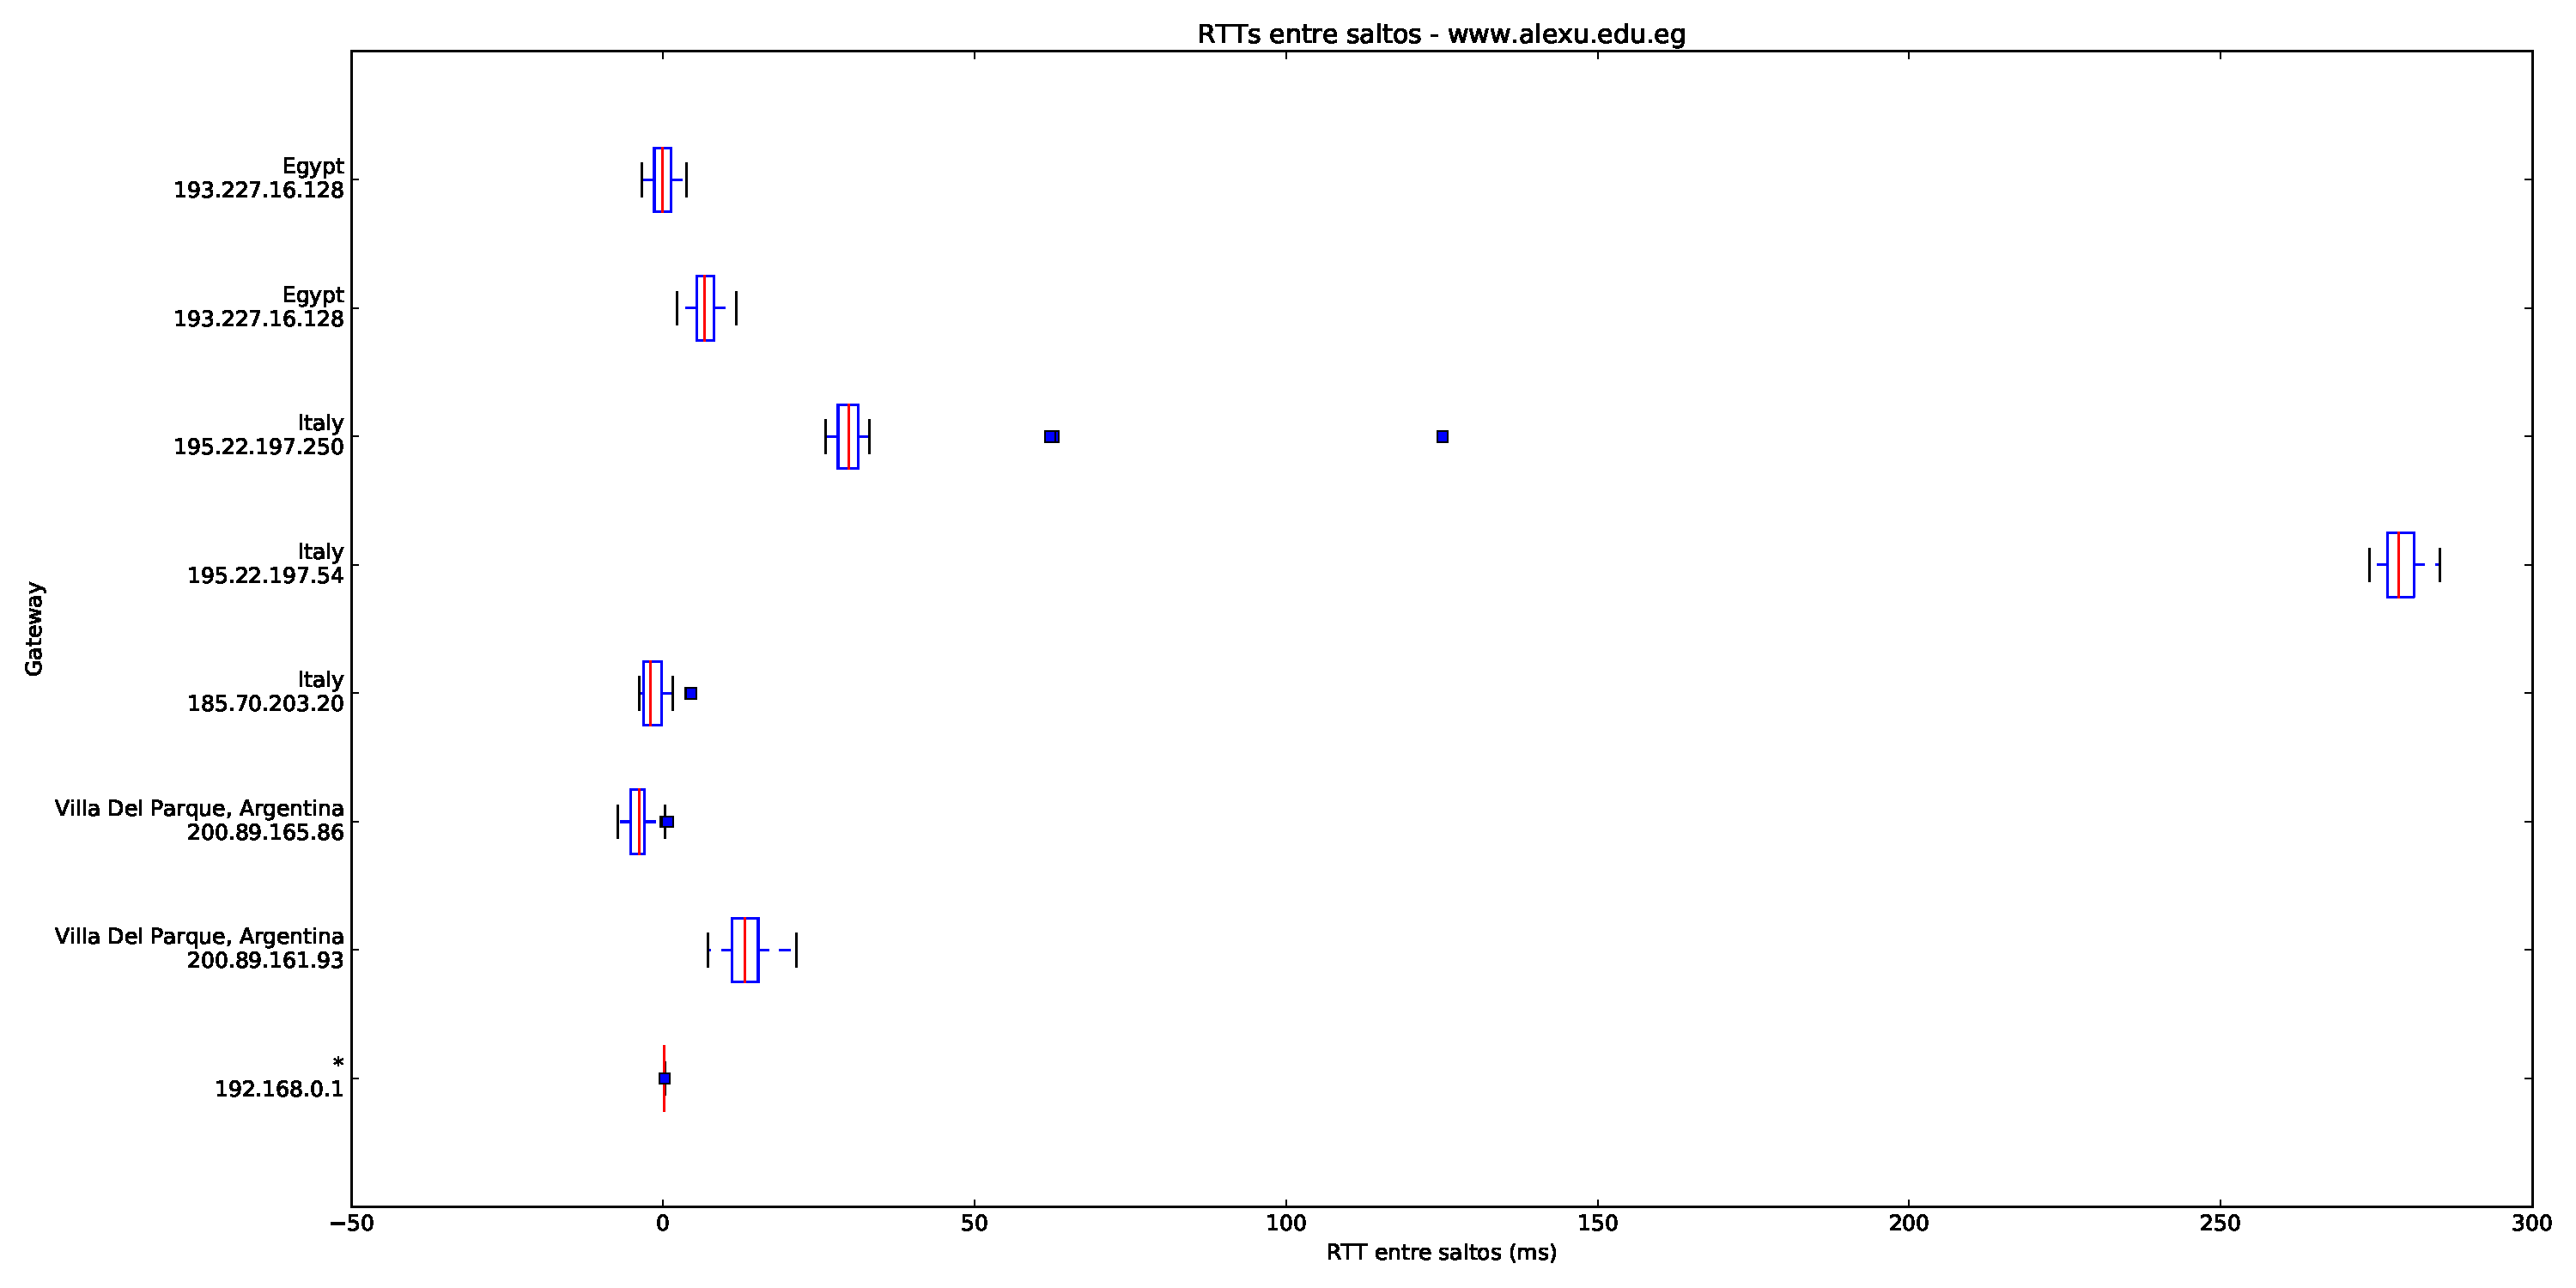
\includegraphics[width=8.5cm]{img/grafico1-www-alexu-edu-eg.pdf}
    \caption{\normalfont RTTs entre saltos. El valor asignado al $i$-ésimo nodo corresponde al salto entre el $i$-ésimo y el $i - 1$-ésimo nodo. Para el primer nodo se utiliza simplemente su RTT.}
\end{figure}

Todas las mediciones son normales en todos los gateways, y no se observan outliers. 

\begin{figure}[H]
    \centering
    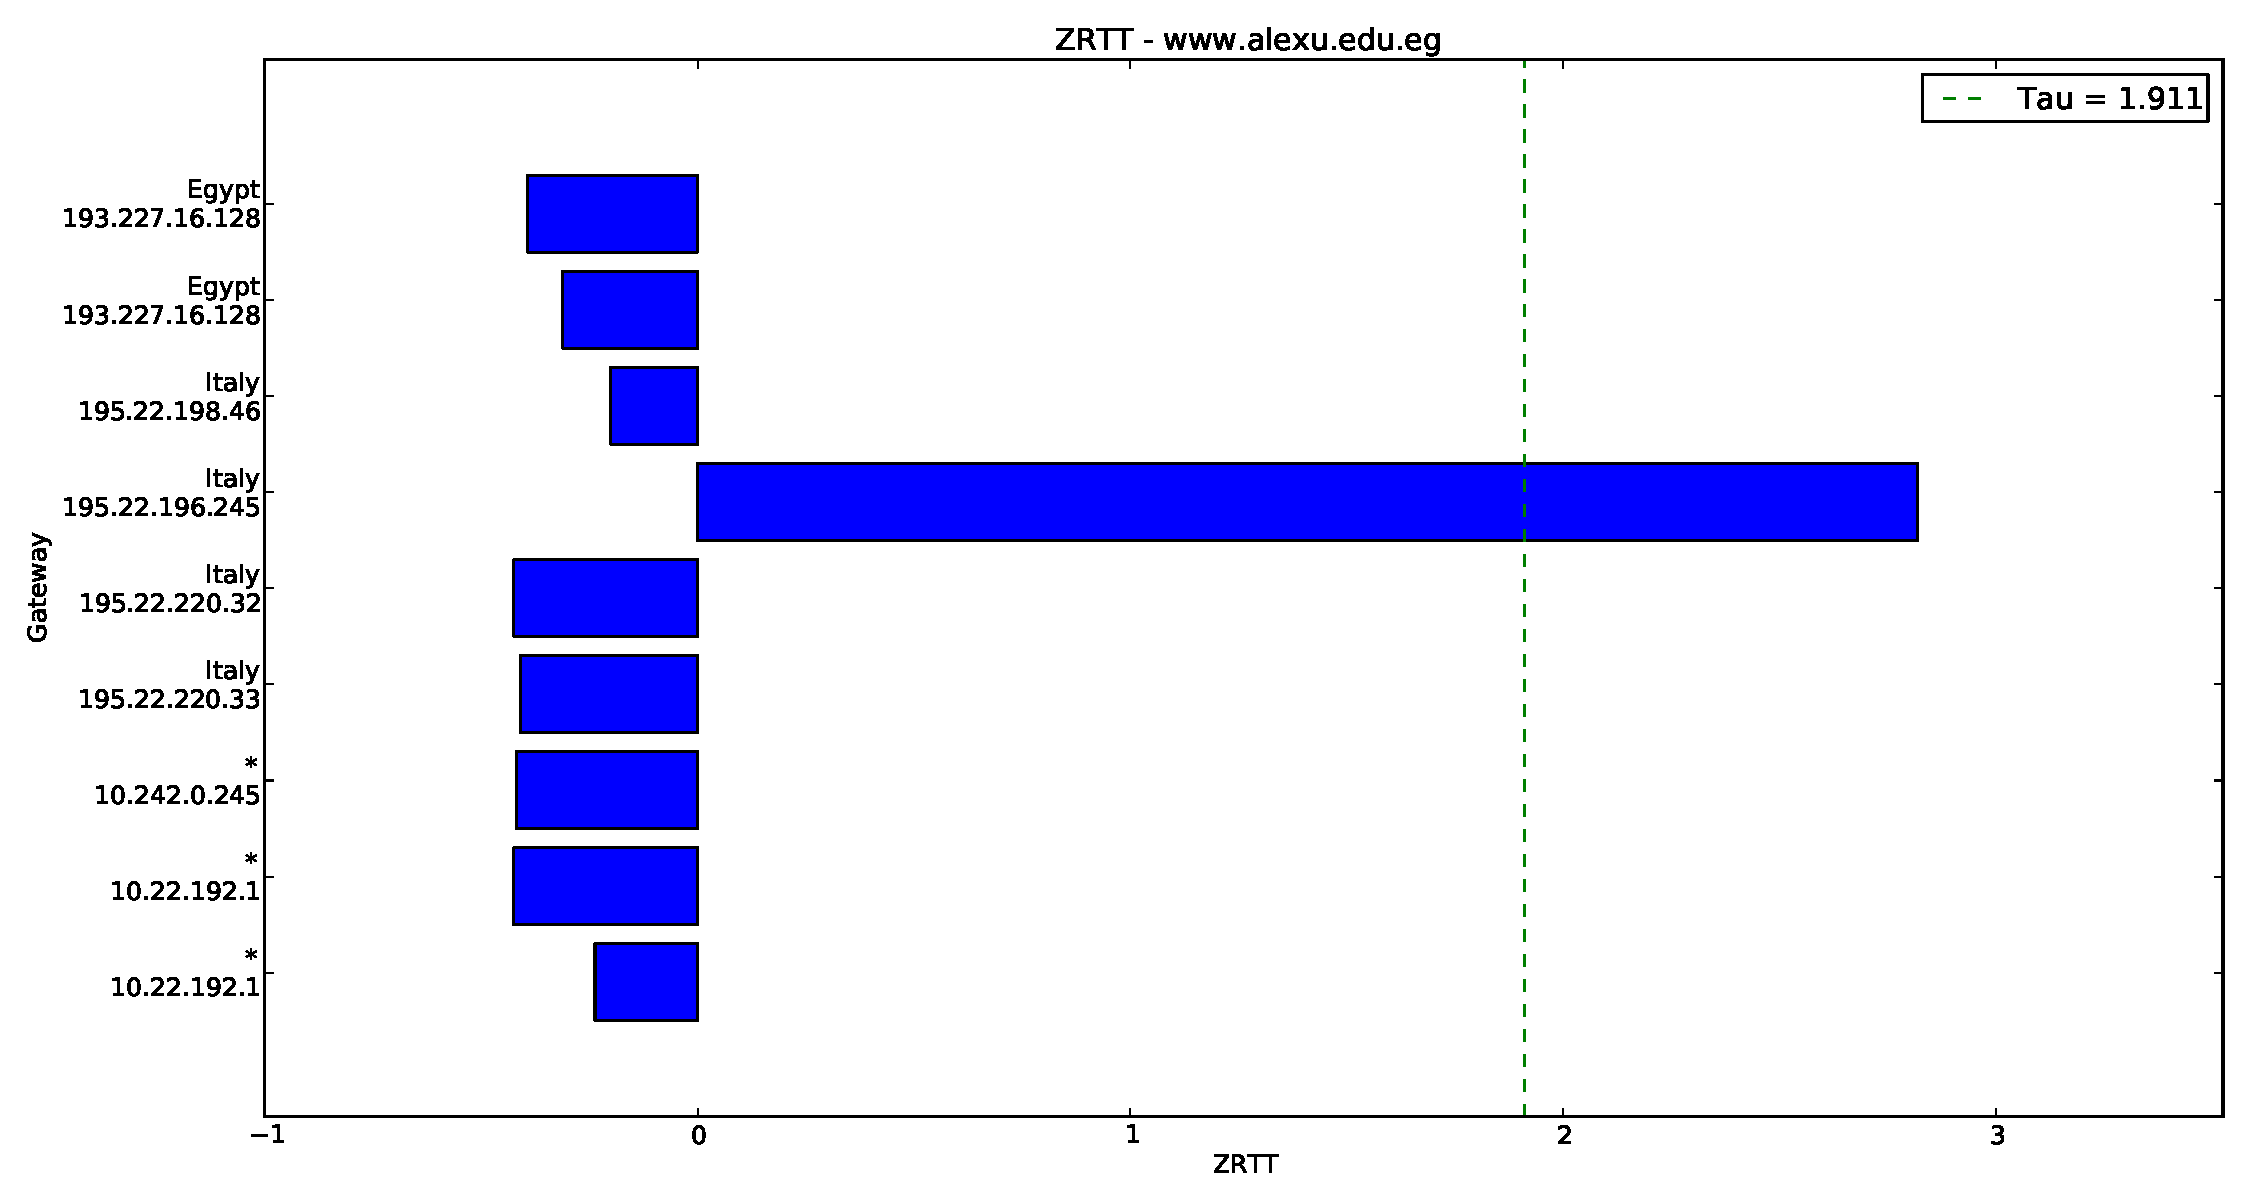
\includegraphics[width=8.5cm]{img/grafico2-www-alexu-edu-eg.pdf}
    \caption{\normalfont ZRTTs entre saltos.}
\end{figure}

En la figura de la ruta hacia Alejandría podemos ver como tenemos problemas de geolocalización. Recién en la segunda IP que corresponde 
a Italia nos está marcando el enlace intercontinental, por lo cuál suponemos que esta primer IP italiana (185.70.203.20) en realidad
se encuentra en Argentina. 

En el traceroute, 9 de los 17 nodos no respondieron el time exceeded (52.9\%).


\begin{figure}[H]
    \centering
    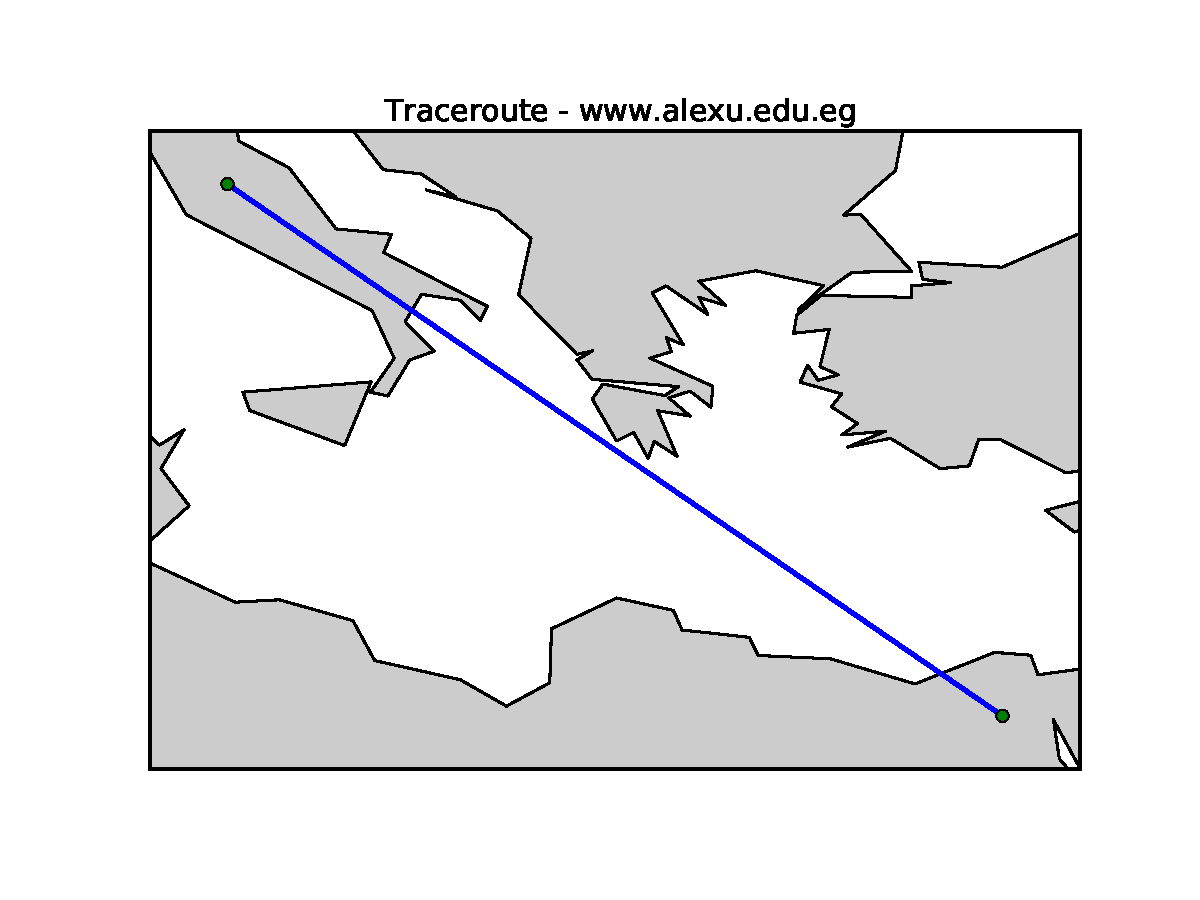
\includegraphics[width=8.5cm]{img/grafico3-www-alexu-edu-eg.pdf}
    \caption{\normalfont Ubicación geográfica estimada de la ruta tomada.}
\end{figure}

En este caso tenemos dos enlaces intercontinentales según muestra el mapa, uno de Argentina hacia Italia, y el segundo de Italia 
hacia Egipto, pero solo detectamos 1 solo enlace, el de Argentina hacia Italia, teniendo así un falso negativo. 
Esto creemos que es debido a la cercanía de Italia con Egipto, a pesar de encontrarse en continentes distintos. 


